\section{The F(AI)\texorpdfstring{\textsuperscript{2}}{2}R Pattern}
\label{sec:pattern}

\subsection{Axes: F(AI)\texorpdfstring{\textsuperscript{2}}{2}R}
\label{sec:axes}

% F(AI)^2R: the four FAIR axes with the (AI) factor multiplied through.
% Visualises the squared-AI claim (\S\ref{sec:axes}) as a 4x2 grid:
% one column per FAIR letter, two rows for the authoring (AI_1) and
% audit (AI_2) passes that the (AI) factor demands per axis.
% Loaded by paper/sections/pattern.tex via \input.
\begin{figure}[!t]
\centering
\begin{tikzpicture}[
  node distance=0pt,
  every node/.style={font=\sffamily\footnotesize, align=center,
                     inner sep=4pt},
  axis/.style={draw, line width=0.5pt, draw=dlrGrau1,
               minimum width=28mm, minimum height=8mm,
               fill=dlrGrau5, text=dlrGrau1, font=\sffamily\bfseries},
  authoring/.style={draw, line width=0.5pt, draw=dlrBlau1,
                    fill=dlrBlau5, text=black,
                    minimum width=28mm, minimum height=12mm,
                    text width=26mm, align=center},
  audit/.style={draw, line width=0.5pt, draw=dlrGruen1,
                fill=dlrGruen5, text=black,
                minimum width=28mm, minimum height=12mm,
                text width=26mm, align=center},
  rowlabel/.style={font=\sffamily\bfseries\footnotesize,
                   text=dlrGrau1, anchor=east, align=right},
]
% Header row: F | A | I | R, on a grey strip
\node[axis] (HF) at (0,0)   {Findable};
\node[axis] (HA) at (3,0)   {Accessible};
\node[axis] (HI) at (6,0)   {Interoperable};
\node[axis] (HR) at (9,0)   {Reusable};

% Authoring row (AI_1)
\node[authoring] (A1) at (0,-1)   {DOI / ORCID;\\IRIs minted};
\node[authoring] (A2) at (3,-1)   {clone-and-build;\\licences};
\node[authoring] (A3) at (6,-1)   {Turtle graph;\\fair2r:\ namespace};
\node[authoring] (A4) at (9,-1)   {prompts;\\Makefile;\\logbook};

% Audit row (AI_2)
\node[audit]    (B1) at (0,-2.2)  {metadata\\agree;\\IRIs unique};
\node[audit]    (B2) at (3,-2.2)  {paywalled\\sources\\vendored};
\node[audit]    (B3) at (6,-2.2)  {Turtle\\validates;\\SHACL};
\node[audit]    (B4) at (9,-2.2)  {clone replays;\\drift\\reported};

% Row labels
\node[rowlabel] at ([xshift=-19mm]A1.west) {(AI)\textsubscript{1}\\authoring pass};
\node[rowlabel] at ([xshift=-19mm]B1.west) {(AI)\textsubscript{2}\\audit pass};

% Top-edge brace label "(AI)^2 multiplied through every axis"
\draw[draw=dlrGrau1, line width=0.4pt]
  ([yshift=4mm]HF.north west) -- ([yshift=4mm]HR.north east);
\node[font=\sffamily\itshape\footnotesize, text=dlrGrau1]
  at ($([yshift=8mm]HF.north west)!0.5!([yshift=8mm]HR.north east)$)
  {(AI)\textsuperscript{2} factor multiplied through every axis};
\end{tikzpicture}
\caption{The F(AI)\textsuperscript{2}R pattern as a $4 \times 2$
grid. The four FAIR axes (top, grey) each carry an authoring pass
$\mathrm{AI}_{1}$ (blue, middle row) and an audit pass
$\mathrm{AI}_{2}$ (green, bottom row); the squared notation is the
typographic commitment that the (AI) factor is multiplied through
every axis rather than appended as a fifth one. Cell contents
summarise \S\ref{sec:axes}; the full mapping is in
Appendix~\ref{app:fair-cells}.}
\label{fig:axes}
\end{figure}


% F(AI)^2R: writers x readers --- the (AI)^2 factor unpacked into the
% four cells of human-or-AI as writer x human-or-AI as reader.
% This figure makes the central distinction of the paper visible at a
% glance: the (AI)^2 factor is squared because both writer and reader
% can be human or AI, and the disclosure surface --- what each cell
% requires from the manuscript bundle --- differs across cells.
% Loaded by paper/sections/pattern.tex via \input, immediately after
% figures/axes which renders the four FAIR axes; this figure renders
% the (AI)^2 factor itself.
\begin{figure}[!t]
\centering
\begin{tikzpicture}[
  every node/.style={font=\sffamily\footnotesize, align=center,
                     inner sep=4pt},
  cell/.style={draw, line width=0.5pt, minimum width=58mm,
               minimum height=24mm, text width=54mm,
               align=left, fill=white, anchor=center,
               draw=dlrGrau1},
  hh/.style={fill=dlrGruen5, draw=dlrGruen1, line width=0.6pt},
  ha/.style={fill=dlrBlau5,  draw=dlrBlau1, line width=0.6pt},
  ah/.style={fill=white,     draw=dlrBlau1, line width=0.6pt, dashed},
  aa/.style={fill=dlrGrau5,  draw=dlrGrau1, line width=0.6pt, dotted},
  axislbl/.style={font=\sffamily\bfseries\footnotesize, text=dlrGrau1,
                  align=center},
  axisrole/.style={font=\sffamily\footnotesize, text=dlrGrau1,
                   align=center, inner sep=2pt},
  cellhdr/.style={font=\sffamily\bfseries\footnotesize, text=black},
  cellsub/.style={font=\sffamily\itshape\footnotesize, text=dlrGrau1},
  cellnote/.style={font=\sffamily\footnotesize, text=black},
  surface/.style={font=\sffamily\footnotesize, text=dlrAccent},
]
% --- Axis labels (writer = top row, reader = left column) ----------
\node[axislbl] at (-3.6, 1.85) {writer};
\node[axisrole, anchor=south] at (-1.55, 1.55) {human};
\node[axisrole, anchor=south] at ( 1.55, 1.55) {AI};
\node[axislbl, rotate=90] at (-5.85, -0.15) {reader};
\node[axisrole, rotate=90, anchor=south] at (-5.55, 1.05)  {human};
\node[axisrole, rotate=90, anchor=south] at (-5.55, -1.45) {AI};

% Hairline rule between the two writer columns / reader rows
\draw[draw=dlrGrau3, line width=0.3pt]
  (-4.50, 1.30) -- (-4.50, -1.55);
\draw[draw=dlrGrau3, line width=0.3pt]
  (-4.95, 1.25) -- (4.65, 1.25);

% --- Cells (2x2) ---------------------------------------------------
% Top-left: human writer, human reader (the classical case)
\node[cell, hh] (HH) at (-1.55, 0.40) {%
  {\cellhdr classical scholarship}\\[1pt]
  {\cellsub all four FAIR axes}\\[2pt]
  {\cellnote prose, citations, manuscript-only;
   transcripts and prompts are out of scope.}};
% Top-right: AI writer, human reader (the paper's primary case)
\node[cell, ha] (AH) at ( 1.55, 0.40) {%
  {\cellhdr LLM-assisted writing}\\[1pt]
  {\cellsub the F(AI)\textsuperscript{2}R primary case}\\[2pt]
  {\cellnote prose + transcripts + prompts + ladder-status +
   per-claim provenance map.}};
% Bottom-left: human writer, AI reader (the audit case)
\node[cell, ah] (HA) at (-1.55, -2.20) {%
  {\cellhdr AI-assisted reading}\\[1pt]
  {\cellsub auditor / scrutinizer / search agent}\\[2pt]
  {\cellnote machine-readable claims, IRIs, SPARQL-able graph;
   licence permits ingestion.}};
% Bottom-right: AI writer, AI reader (the systemic case)
\node[cell, aa] (AA) at ( 1.55, -2.20) {%
  {\cellhdr AI-to-AI corpus}\\[1pt]
  {\cellsub training data / ML retrieval / agent-mediated review}\\[2pt]
  {\cellnote everything above, plus base-rate disclosure on the
   training-set side; collapse risk.}};

% --- Disclosure-surface labels (right edge) ------------------------
\node[surface, anchor=west] at (4.85,  0.40)
  {\textbf{disclosure surface:}\\\textit{paper bundle widens}\\\textit{top-left $\to$ bottom-right}};

% --- Caption-ready footer band -------------------------------------
\node[font=\sffamily\itshape\footnotesize, text=dlrGrau1,
      anchor=west, align=left]
  at (-4.95, -3.85)
  {The (AI) factor squared: both writer and reader can be human or AI.
   The paper's primary case is the top-right cell; its auditability
   premise is that bottom-left and bottom-right are coming next.};
\end{tikzpicture}
\caption{The (AI)\textsuperscript{2} factor unpacked as a $2\times 2$
grid of writer (columns) and reader (rows). The top-left cell
(human writer, human reader) is the classical scholarly case and
needs only the manuscript proper; the top-right cell (AI writer,
human reader) is this paper's primary case and is what every
practice in \S\ref{sec:eight} addresses; the bottom-left cell (human
writer, AI reader) is the audit / scrutinizer / agent-mediated
search case and requires machine-readable claims and a SPARQL-able
provenance graph; the bottom-right cell (AI writer, AI reader) is
the systemic case --- training-data ingestion, agent-to-agent
review, autonomous literature search --- and additionally requires
base-rate disclosure on the training-set side. The disclosure
surface widens monotonically along the diagonal: top-left needs
only prose and citations, bottom-right needs the full
F(AI)\textsuperscript{2}R bundle.}
\label{fig:ai-squared-grid}
\end{figure}


We retain the four canonical FAIR axes and read each in two passes
(Figure~\ref{fig:axes}). The (AI)\textsuperscript{2} factor itself
unpacks into the four cells of writer-vs-reader
(Figure~\ref{fig:ai-squared-grid}): a manuscript that will be both
written and read by humans only needs the manuscript proper, while a
manuscript whose readers include AI agents needs every artefact in
the F(AI)\textsuperscript{2}R bundle. The authoring pass (AI\textsubscript{1})
produces the artefact for that axis. The audit pass
(AI\textsubscript{2}) verifies the artefact against the axis after
the fact, never in the same role and never in the same commit. The
two passes are what justifies the squared notation. The (AI) factor
is multiplied through every axis.

\paragraph{F.}
Authoring mints persistent identifiers (DOI via Zenodo, ORCID for
authors), populates machine-readable metadata
(\texttt{CITATION.cff}, \texttt{codemeta.json},
\texttt{.zenodo.json}), and assigns IRIs to per-claim entities. Audit
verifies the metadata surfaces agree, no IRI is dangling, and every
manuscript-cited claim has a graph entry.

\paragraph{A.}
Authoring clones-and-builds: a third party with the public repository
and a documented toolchain reproduces the PDF. Audit verifies the
licence pair (MIT for code/RDF, CC-BY-4.0 for prose), that paywalled
sources have been vendored where licensable, and that the redaction
policy covers what it claims.

\paragraph{I.}
Authoring commits the provenance graph as PROV-O over Turtle in
\texttt{doc/provenance.ttl}. Audit validates the Turtle, runs SHACL
shapes if defined, and verifies every section has a
\texttt{prov:Activity} record that produced it.

\paragraph{R.}
Authoring commits the per-role prompts under \texttt{agents/}, the
build target under \texttt{paper/Makefile}, and the logbook under
\texttt{doc/logbook.md}. Audit replays the pipeline on a clean clone
and reports drift.

\subsection{The pipeline as the team}
\label{sec:pipeline}

% Ten-stage F(AI)^2R agent pipeline. Self-contained TikZ figure.
% Loaded by paper/sections/pattern.tex via \input.
\begin{figure*}[!t]
\centering
\begin{tikzpicture}[
  node distance=4mm and 4mm,
  every node/.style={font=\sffamily\footnotesize, align=center,
                     inner sep=4pt, minimum height=8mm},
  authoring/.style={draw, rectangle, fill=dlrBlau5, draw=dlrBlau1,
                    line width=0.5pt, text=black, minimum width=22mm},
  audit/.style={draw, rectangle, fill=dlrGruen5, draw=dlrGruen1,
                line width=0.5pt, text=black, minimum width=22mm},
  curate/.style={draw, rectangle, fill=dlrGelb5, draw=dlrGelb1,
                 line width=0.5pt, text=black, minimum width=22mm},
  orchestrator/.style={draw, rectangle, fill=dlrGrau5,
                       draw=dlrGrau1, line width=0.5pt, text=dlrGrau1,
                       minimum width=22mm},
  arrow/.style={-{Latex[length=1.5mm]}, draw=dlrGrau1, line width=0.4pt},
  legend/.style={font=\sffamily\scriptsize, text=dlrGrau1},
]
% Row 1: orchestrator + authoring stages (left to right)
\node[orchestrator] (orc)  {0. Orchestrator};
\node[authoring, right=of orc] (res)  {1. Research};
\node[authoring, right=of res] (sa)   {1.5. Source\\Analyzer};
\node[authoring, right=of sa]  (sw)   {2. Scientific\\Writer};
\node[authoring, right=of sw]  (ill)  {3. Illustration};

% Row 2: audit stages (right to left below)
\node[audit, below=10mm of ill] (lay)  {4. Layout\\Scrutinizer};
\node[audit, left=of lay]  (read) {5. Readability\\\& Novelty};
\node[audit, left=of read] (ali)  {6. Aligner\\(FAIR)};
\node[curate, left=of ali] (pc)   {7. Provenance\\Curator};
\node[orchestrator, left=of pc] (site) {8. Site Agent};

% Authoring flow (row 1, left → right)
\draw[arrow] (orc) -- (res);
\draw[arrow] (res) -- (sa);
\draw[arrow] (sa)  -- (sw);
\draw[arrow] (sw)  -- (ill);

% Authoring → Audit transition
\draw[arrow] (ill.south) |- ([yshift=2mm]lay.north);

% Audit flow (row 2, right → left)
\draw[arrow] (lay)  -- (read);
\draw[arrow] (read) -- (ali);
\draw[arrow] (ali)  -- (pc);
\draw[arrow] (pc)   -- (site);

% Handback edges (audit → orchestrator), dashed
\draw[arrow, dashed, draw=dlrGrau3]
  (lay.south) to[bend right=20] node[legend, below, midway]
    {hand-back} (orc.south);

% Legend
\node[legend, anchor=north west, draw=dlrGrau4, fill=white,
      inner sep=4pt]
  at ([xshift=0mm, yshift=-2mm]lay.south west)
  {%
    \tikz\draw[fill=dlrBlau5, draw=dlrBlau1] (0,0) rectangle (3mm,3mm);\,Authoring \quad
    \tikz\draw[fill=dlrGruen5, draw=dlrGruen1] (0,0) rectangle (3mm,3mm);\,Audit \quad
    \tikz\draw[fill=dlrGelb5, draw=dlrGelb1] (0,0) rectangle (3mm,3mm);\,Curate \quad
    \tikz\draw[fill=dlrGrau5, draw=dlrGrau1] (0,0) rectangle (3mm,3mm);\,Orchestration / Site
  };
\end{tikzpicture}
\caption{The ten-stage F(AI)\textsuperscript{2}R pipeline. Authoring
(blue) and audit (green) stages are strictly separated by the
handback discipline (\S\ref{sec:handback}); only the Provenance
Curator (yellow) writes \texttt{doc/provenance.ttl}; the Orchestrator
and Site Agent (grey) are coordination roles that never edit prose.
A scrutinizing stage that finds a defect files a \emph{handback} (dashed
arrow) rather than patching in place.}
\label{fig:pipeline}
\end{figure*}


Ten stages, coordinated by an Orchestrator, with strict handback
between prose-owning and audit-owning agents
(Figure~\ref{fig:pipeline}):

\begin{description}[leftmargin=1.2em,itemsep=2pt]
    \item[0. Orchestrator.] Inspects state, dispatches one downstream
        stage at a time. Never edits prose.
    \item[1. Research.] Per-section literature audit. Produces sources
        and transcripts under \texttt{doc/sources/} and
        \texttt{doc/transcripts/}.
    \item[1.5. Source Analyzer.] Promotes
        \textsc{lit-retrieved}\,$\to$\,\textsc{ai-confirmed}; never crosses into
        \textsc{lit-read}.
    \item[2. Scientific Writer.] Owns prose, register, \LaTeX. Does
        not change claims or introduce citations without a verified
        source.
    \item[3. Illustration.] Owns figures; halts on load-bearing values
        still at \textsc{lit-retrieved}.
    \item[4. Layout Scrutinizer.] Reads the rendered PDF, files a
        Layout Defect Registry under \texttt{doc/handbacks/}.
    \item[5. Readability \& Novelty Scrutinizer.] Reads the markdown,
        flags repetition, list-of-lists prose, hedging chains, and
        unsupported novelty. Files a registry.
    \item[6. Aligner (FAIR).] Audits traceability across paper,
        sources, README, and registries. Routes hand-backs; never
        edits content.
    \item[7. Provenance Curator.] Sole writer of
        \texttt{doc/provenance.ttl}; refuses to invent triples.
    \item[8. Site Agent.] Owns the public site; refuses to render
        without explicit publication consent. The site never
        introduces a new claim.
\end{description}

The agent that owns prose cannot mark its own claims as verified. The
agent that audits layout cannot edit prose. The agent that curates
provenance cannot write \LaTeX. \emph{Specialisation reduces
hallucination at the seam.}

\subsection{The verification ladder as an FSM}
\label{sec:ladder}

% F(AI)^2R verification ladder as a finite-state machine.
% Source of truth: paper/figures/ladder-fsm.mmd (Mermaid stateDiagram).
% Build: rendered to paper/figures/ladder-fsm.pdf via mmdc; the
% Pages site renders the same .mmd client-side via mermaid.min.js so
% paper and site stay in lock-step. See paper/figures/ladder-fsm.figspec.md.
% This .tex shim is what % F(AI)^2R verification ladder as a finite-state machine.
% Source of truth: paper/figures/ladder-fsm.mmd (Mermaid stateDiagram).
% Build: rendered to paper/figures/ladder-fsm.pdf via mmdc; the
% Pages site renders the same .mmd client-side via mermaid.min.js so
% paper and site stay in lock-step. See paper/figures/ladder-fsm.figspec.md.
% This .tex shim is what % F(AI)^2R verification ladder as a finite-state machine.
% Source of truth: paper/figures/ladder-fsm.mmd (Mermaid stateDiagram).
% Build: rendered to paper/figures/ladder-fsm.pdf via mmdc; the
% Pages site renders the same .mmd client-side via mermaid.min.js so
% paper and site stay in lock-step. See paper/figures/ladder-fsm.figspec.md.
% This .tex shim is what \input{figures/ladder-fsm} from
% paper/sections/pattern.tex resolves to: it wraps the rendered PDF
% in a figure float with the manuscript caption.
\begin{figure}[!t]
\centering
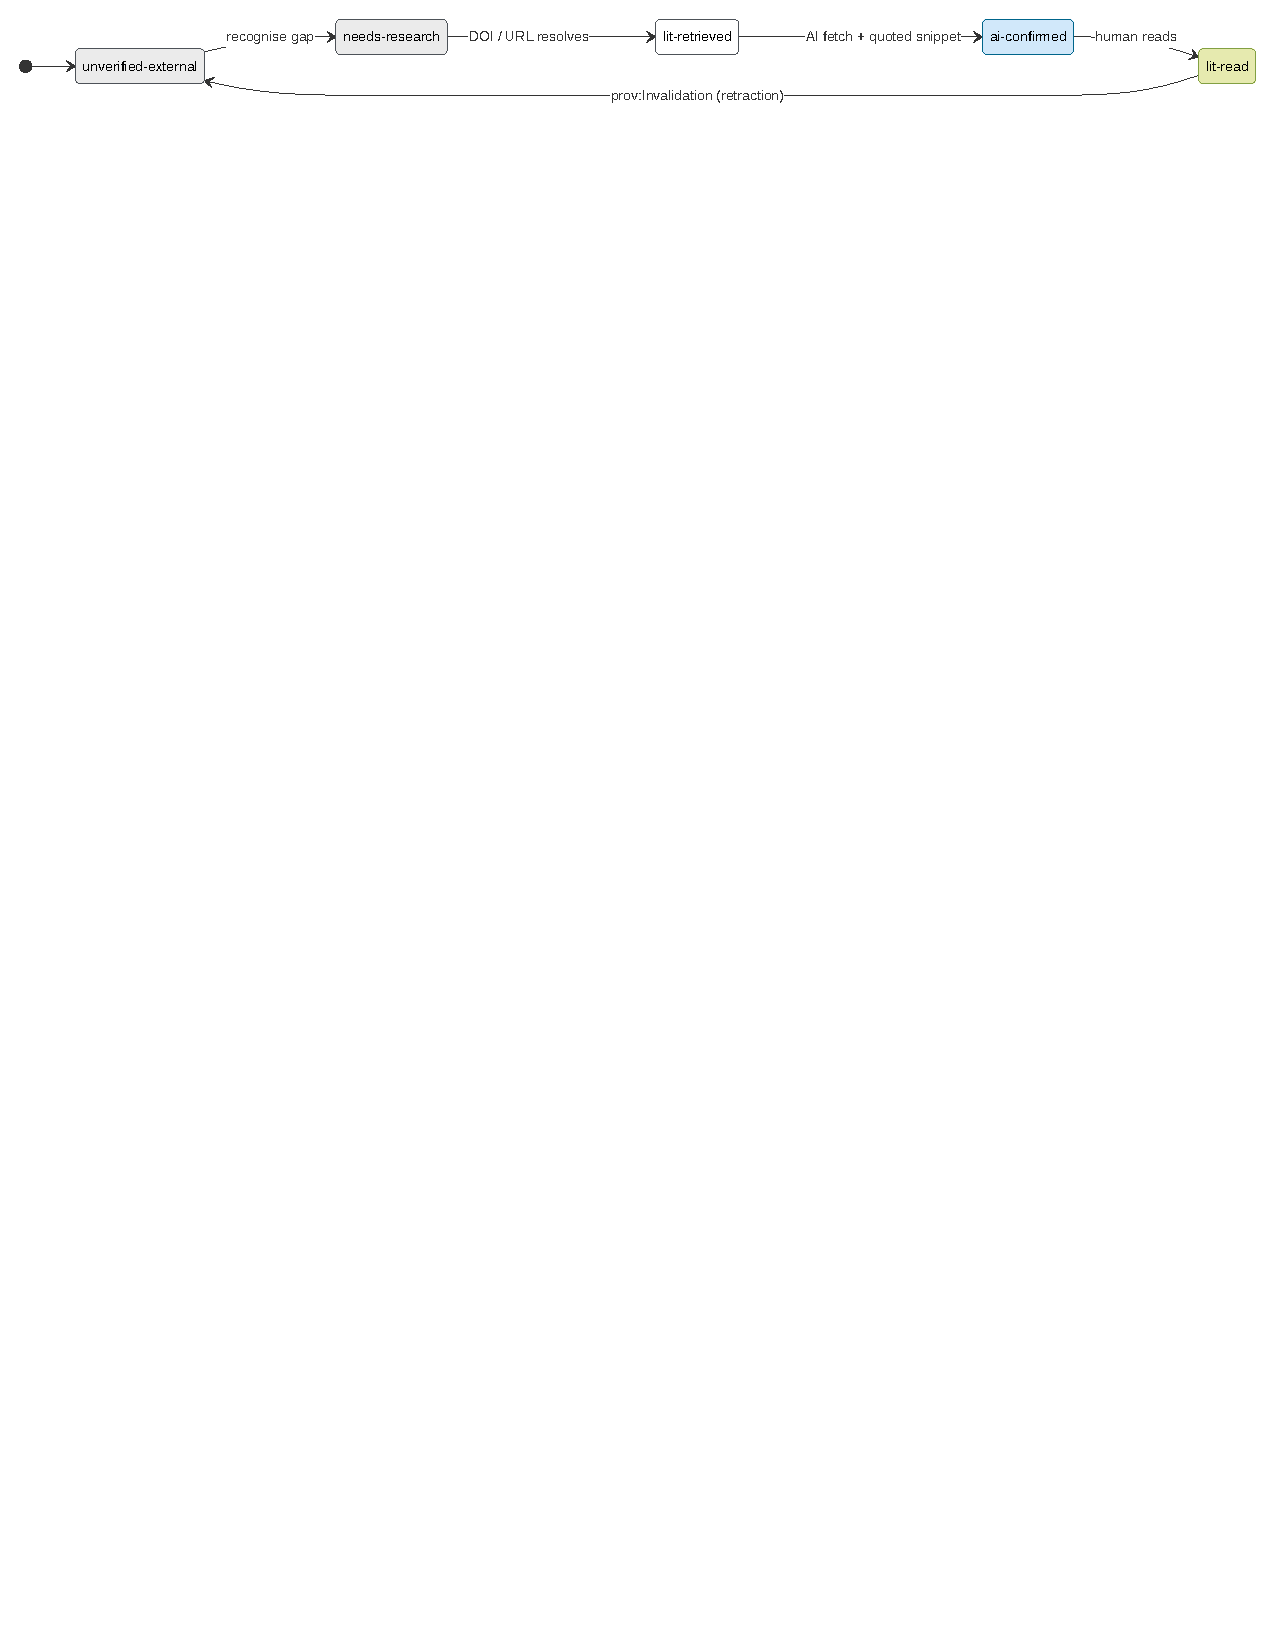
\includegraphics[width=0.92\linewidth]{figures/ladder-fsm.pdf}
\caption{The verification ladder as a finite-state machine. A
\texttt{fair2r:Claim} progresses left-to-right as evidence
accumulates; \textsc{ai-confirmed} is the ceiling an LLM agent can
deliver on its own (\S\ref{sec:ladder}). Retraction is the only
back-edge and is recorded as a \texttt{prov:Invalidation} activity
in \texttt{doc/provenance.ttl}, never as a deletion. A claim may be
\emph{invoked} at its current rung or below; load-bearing or
contested claims still require \textsc{lit-read}. Source: Mermaid
\texttt{stateDiagram-v2} at \texttt{paper/figures/ladder-fsm.mmd},
mirrored on the public site.}
\label{fig:ladder-fsm}
\end{figure}
 from
% paper/sections/pattern.tex resolves to: it wraps the rendered PDF
% in a figure float with the manuscript caption.
\begin{figure}[!t]
\centering
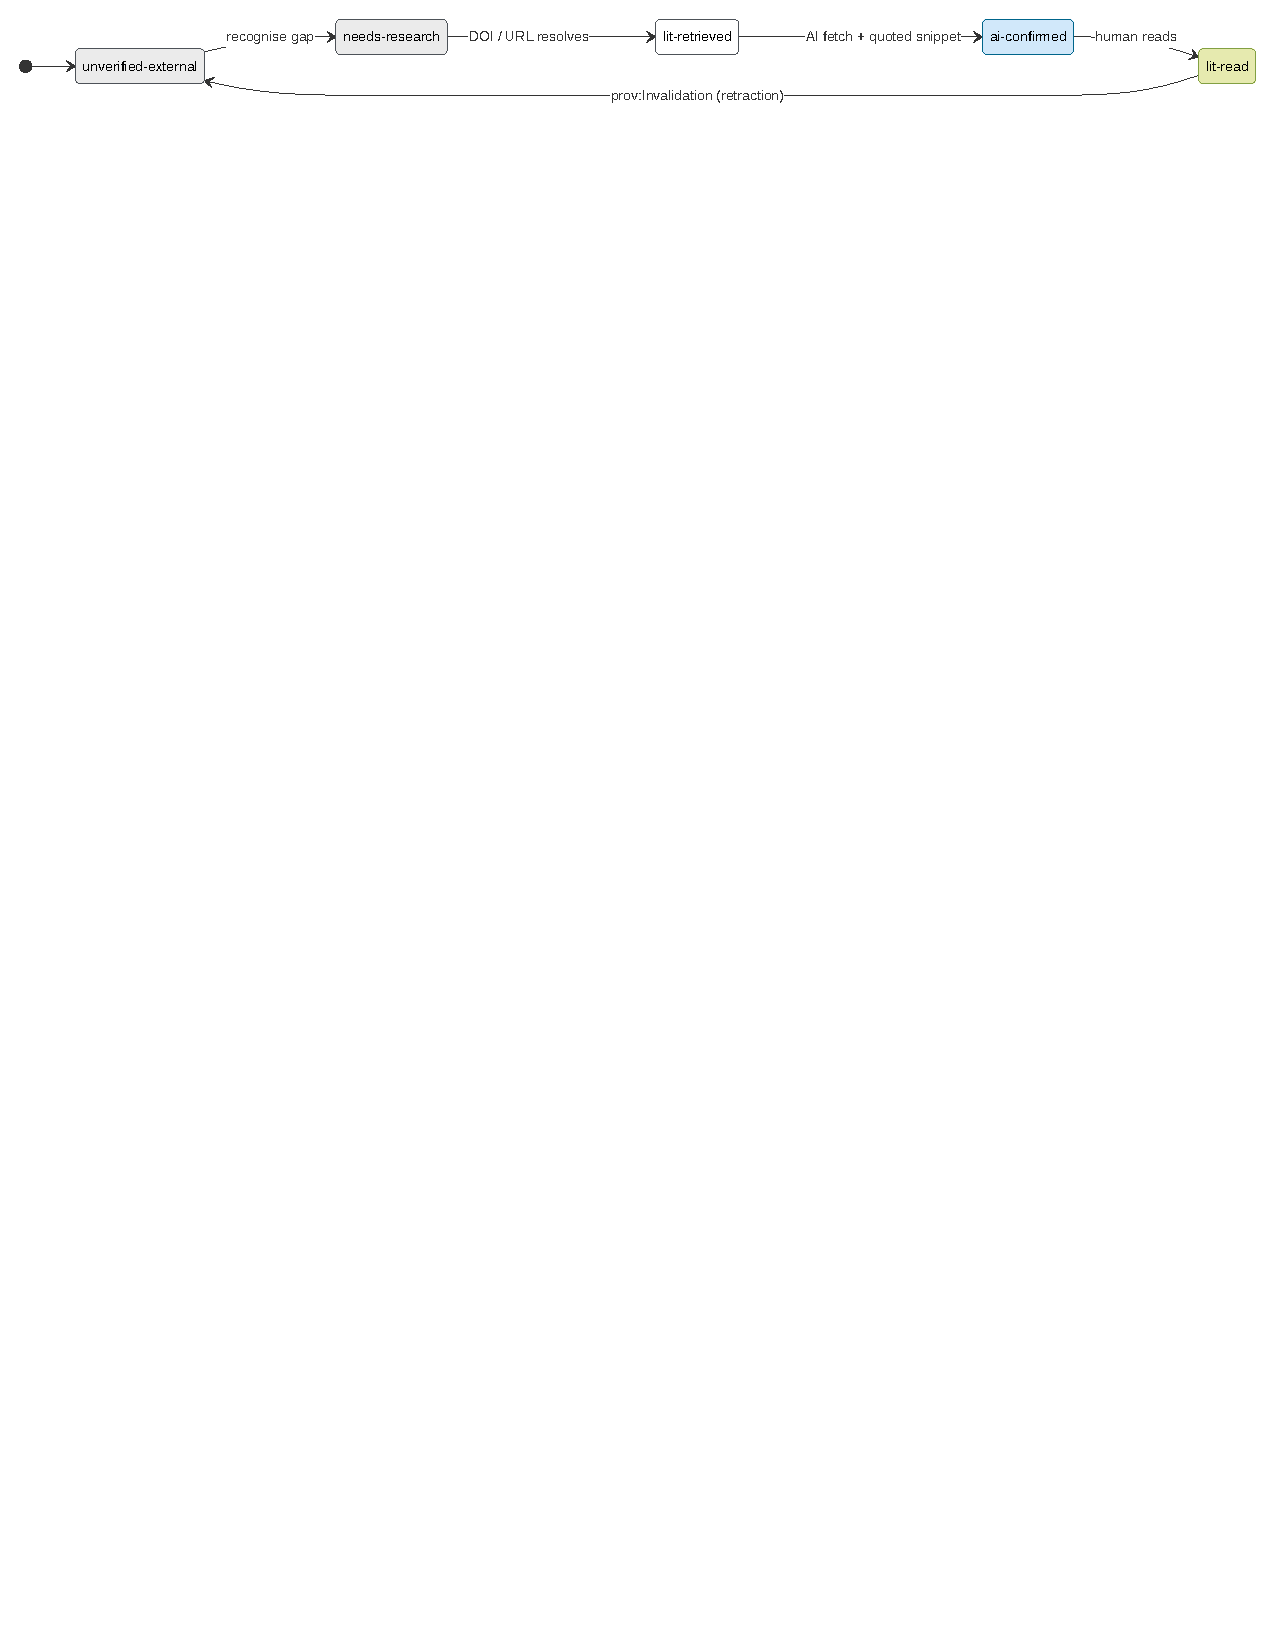
\includegraphics[width=0.92\linewidth]{figures/ladder-fsm.pdf}
\caption{The verification ladder as a finite-state machine. A
\texttt{fair2r:Claim} progresses left-to-right as evidence
accumulates; \textsc{ai-confirmed} is the ceiling an LLM agent can
deliver on its own (\S\ref{sec:ladder}). Retraction is the only
back-edge and is recorded as a \texttt{prov:Invalidation} activity
in \texttt{doc/provenance.ttl}, never as a deletion. A claim may be
\emph{invoked} at its current rung or below; load-bearing or
contested claims still require \textsc{lit-read}. Source: Mermaid
\texttt{stateDiagram-v2} at \texttt{paper/figures/ladder-fsm.mmd},
mirrored on the public site.}
\label{fig:ladder-fsm}
\end{figure}
 from
% paper/sections/pattern.tex resolves to: it wraps the rendered PDF
% in a figure float with the manuscript caption.
\begin{figure}[!t]
\centering
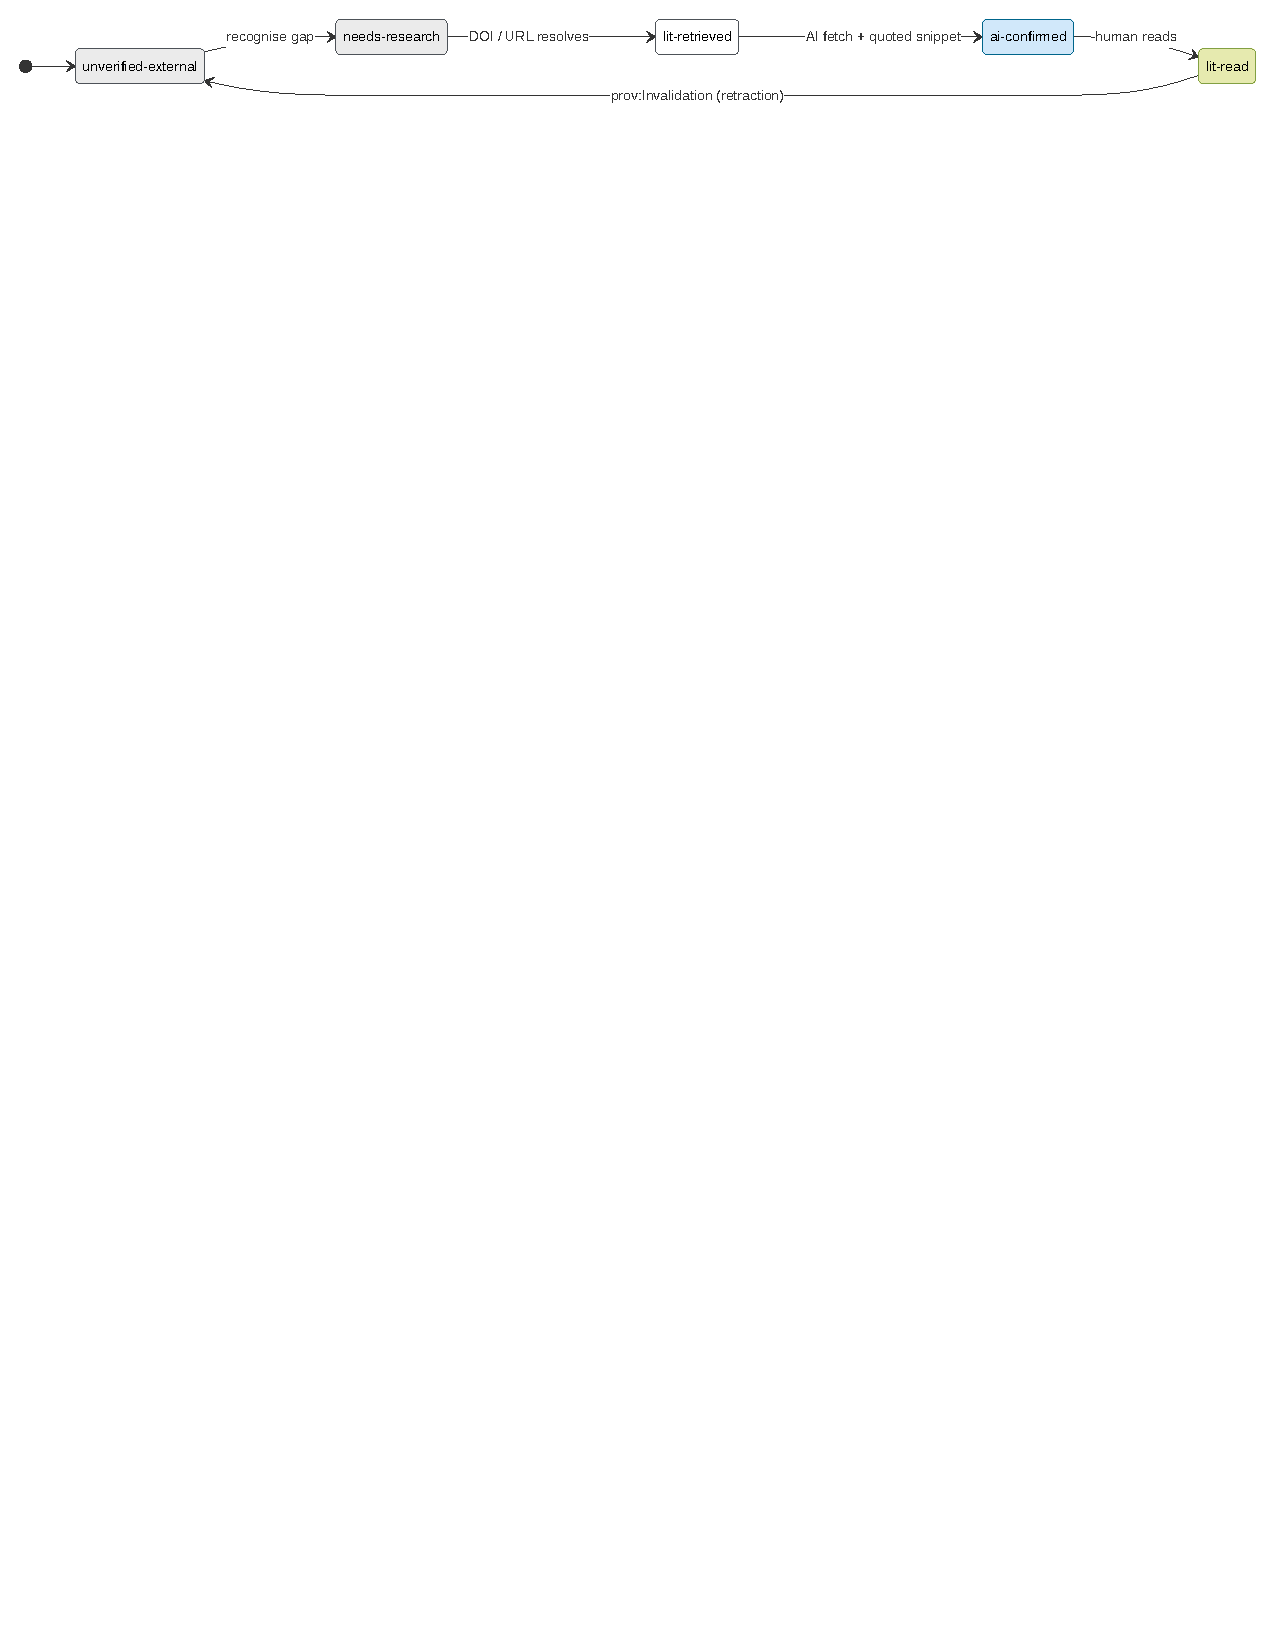
\includegraphics[width=0.92\linewidth]{figures/ladder-fsm.pdf}
\caption{The verification ladder as a finite-state machine. A
\texttt{fair2r:Claim} progresses left-to-right as evidence
accumulates; \textsc{ai-confirmed} is the ceiling an LLM agent can
deliver on its own (\S\ref{sec:ladder}). Retraction is the only
back-edge and is recorded as a \texttt{prov:Invalidation} activity
in \texttt{doc/provenance.ttl}, never as a deletion. A claim may be
\emph{invoked} at its current rung or below; load-bearing or
contested claims still require \textsc{lit-read}. Source: Mermaid
\texttt{stateDiagram-v2} at \texttt{paper/figures/ladder-fsm.mmd},
mirrored on the public site.}
\label{fig:ladder-fsm}
\end{figure}


Every claim carries a verification state. The states are organised
as a finite-state machine (Figure~\ref{fig:ladder-fsm}), monotone
non-decreasing modulo explicit retraction:

\begin{quote}\small
\textsc{unverified-external}
\(\to\) \textsc{needs-research}
\(\to\) \textsc{lit-retrieved}
\(\to\) \textsc{ai-confirmed}
\(\to\) \textsc{lit-read}
\end{quote}

\noindent \textsc{lit-retrieved}: a candidate URL or DOI that
resolves. \textsc{ai-confirmed}: an AI agent has read the source and
confirmed it supports the claim, with a quoted snippet preserved in
\texttt{doc/sources.md}. \textsc{lit-read}: a human has read the
source and confirmed both that it supports the claim and that the
inference from source to claim is sound. A claim may invoke a source
at its current rung or below; load-bearing or contested claims still
require \textsc{lit-read}.

The \textsc{ai-confirmed} rung exists because verification overhead
is real and dominates writer cycles. Most retrieved entries are
obvious from the abstract; a small minority anchor contested claims;
the single-tier gate forced the human reader through both populations
at the same cost. Splitting the work between the Source Analyzer
(cheap) and the human (expensive) is the lever that makes the
practice economically tenable.

\paragraph{Crosswalk.} Retrieval depth maps to PRISMA 2020:
\textsc{lit-retrieved}\,=\,Identification, \textsc{ai-confirmed}\,=\,Screening,
\textsc{lit-read}\,=\,Included. Invocation strength maps to GRADE: a
claim invoked at \textsc{lit-read} carries a GRADE certainty floor of
\textsc{moderate}; a claim at \textsc{ai-confirmed} can carry at most
\textsc{low}. The mapping is a floor, not a ceiling.

\subsection{Handback discipline}
\label{sec:handback}

The four scrutinizing stages --- Source Analyzer, Layout Scrutinizer,
Readability \& Novelty Scrutinizer, Aligner --- never edit source.
They write \emph{Defect Registries} under
\texttt{doc/handbacks/}; the repair lands in a subsequent commit by
a prose-owning agent. The cost is one extra commit boundary per
cycle. The payoff is that ``what did the scrutinizer actually flag?''
has a single canonical answer in the git history. The mirror
discipline that backs the handback --- every primary artefact has
a (source, render) pair under version control, the build either
agrees or fails --- is enumerated as practice~4 of \S\ref{sec:eight}.



\noindent The pattern composes with two forward-looking
extensions --- domain ontologies (SOSA / SSN, OM-2 / QUDT) for
sub-discipline value semantics, and provenance-graph
interconnectivity (the bioinformatics precedent under data-volume
pressure, restated for LLM-assisted scholarship) --- recorded in
Appendix~\ref{sec:appendix-pattern-extensions}. Both are off the
critical path of the eight integrated practices but are how
F(AI)\textsuperscript{2}R generalises beyond the present case.

\paragraph{Cousins.}
Read structurally, F(AI)\textsuperscript{2}R borrows more from
formal methods than from the data-management literature. Each
\texttt{fair2r:Claim} IRI is a conjecture; the verification ladder
is a proof-state machine; the audit pass is a proof-checker that
verifies structural properties of the graph rather than
re-discovering them; the SHACL shapes
(Appendix~\ref{sec:appendix-pattern-extensions}) are invariants;
the handback discipline is the prover / checker separation that
model checking and certified-software efforts treat as
load-bearing~\cite{clarke2009modelchecking,klein2009sel4}\todo[inline]{verify}.
The analogy is partial --- a manuscript is not a transition
system, and \textsc{lit-read} is not soundness --- but the
imports it suggests (counter-example witnesses on retracted claims;
lemma libraries of vetted claims that successor papers can cite by
IRI without re-verifying) are flagged as future work.
